\documentclass[12pt]{article}

\usepackage{amsmath}
\usepackage{array}
\usepackage{caption}
\usepackage[top=1in, bottom=1in, left=0.75in, right=0.75in]{geometry}
\usepackage{graphicx}
\usepackage[colorlinks=true, allcolors=blue]{hyperref}
\usepackage[utf8]{inputenc}
\usepackage{minted}
\usepackage{multirow}
\usepackage{nameref}
\usepackage{pdfpages}
\usepackage[section]{placeins}

\graphicspath{{figures/}}

\begin{document}

\begin{titlepage}
  \begin{center} \LARGE
    \vspace*{1.5in}

    ECE 272 Lab 5

    Fall 2018

    \vfill

    Serial Peripheral Interface (SPI)

    Phi Luu

    \vfill

    November 14\textsuperscript{th}, 2018

    Grading TA: Edgar Perez

    Lab Partner: Benjamin Geyer

    \vspace{1.5in}
  \end{center}
\end{titlepage}

%%%%%%%%%%%%%%%%%%%%%%%%%%%%%%%%%%%%%%%%%%%%%%%%%%%%%%%%%%%%%%%%%%%%%%%%%%%%%%%%
% Introduction
%%%%%%%%%%%%%%%%%%%%%%%%%%%%%%%%%%%%%%%%%%%%%%%%%%%%%%%%%%%%%%%%%%%%%%%%%%%%%%%%
\section{Introduction}

\textit{Serial Peripheral Interface} (\textit{SPI}) is a method of transmitting multiple bits of data using minimal hardware. When two pieces of hardware communicates with each other via SPI, they need to share a clock. At every rising edge of the clock, the data is transmitted from one device to the other.

\begin{figure}[ht]
  \centering
  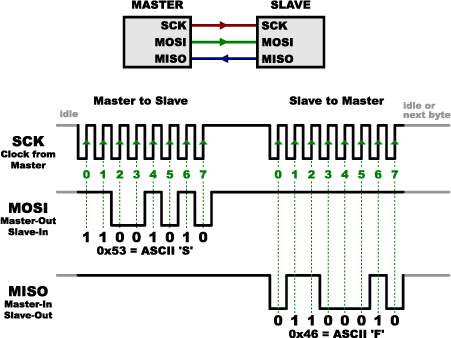
\includegraphics[width=0.75\textwidth]{spi.png}
  \caption{The waveform diagram of the master and the slave in SPI communication protocol \cite{SparkFunSpi}}
  \label{figure:1}
\end{figure}

In Figure~\ref{figure:1}, at every rising edge of $SCK$ (clock from master), the data $MOSI$ (master-out slave-in) is transmitted from the master device to the slave device. After 8 rising edges, an 8-bit data will have been transmitted---in this case, $11001010$ from master to slave.

When the data goes over the designated number of bits, in this case 8 bits, the SPI will always ``forget" the left most bit and transmit the latest chunk of bits.

In this lab, I and Ben designed a SPI protocol using the DE10-Lite FPGA. We used a button as a clock signal, a switch as the data line, and six seven-segment displays as the indicator of the data transmission from the SPI.

%%%%%%%%%%%%%%%%%%%%%%%%%%%%%%%%%%%%%%%%%%%%%%%%%%%%%%%%%%%%%%%%%%%%%%%%%%%%%%%%
% Design
%%%%%%%%%%%%%%%%%%%%%%%%%%%%%%%%%%%%%%%%%%%%%%%%%%%%%%%%%%%%%%%%%%%%%%%%%%%%%%%%
\section{Design}

The system takes in two inputs: one for the clock signal, controlled by a push button, and one for the data, controlled by a switch. This 2-bit input then goes to the SPI. The SPI protocol always outputs an 8-bit binary into a parser to pass into a seven-segment display decoder. Finally, the decoder outputs to the LEDs, indicating the current data being transmitted by the SPI protocol, as illustrated by the block diagram in Figure~\ref{figure:2} below.

\begin{figure}[ht]
  \centering
  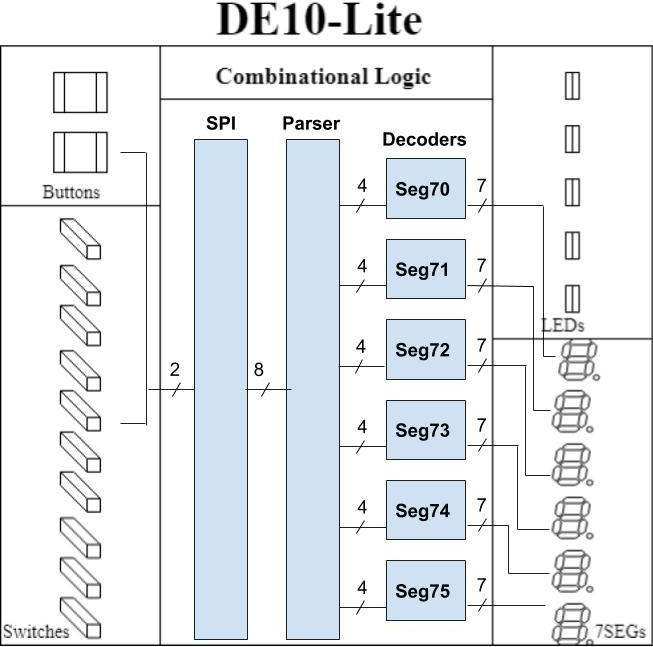
\includegraphics[width=0.75\textwidth]{lab5_block_diagram.png}
  \caption{Block diagram}
  \label{figure:2}
\end{figure}

The SPI module takes in the clock signal and the data. It outputs an 8-bit to the parser, and every time the clock rises, it shifts the current value of the output 1 bit to the left and then add the input bit (data) to the right.

\begin{equation} \label{equation:1}
  output = (output << 1) + data
\end{equation}

For example, let the initial value of the output is $00000000$, if the data is $1$ when the clock rises, the output then becomes

\begin{equation} \label{equation:2}
  output = (00000000 << 1) + 1 = 00000001
\end{equation}

Suppose for the next 7 times the clock rises, the data is $1100110$, then $output = 11100110$.

If the clock rises again, $output$ will be overflow. In this case, the SPI will ``forget" the oldest bit (the most significant bit), the first $1$. Suppose when the clock rises again, the data is a $1$. Then, $output = 11001101$.

The SPI module has the same design as explained above. We reuse the parser and the decoder modules, thus there is nothing new in these modules. However, for the sake of clarity, I will explain the functionality of the parser and the decoder below.

The parser takes in an 8-bit binary number, and SystemVerilog automatically converts numbers between binary, hex, and decimal systems. Since the SPI result is always an 8-bit number, its maximum value is a 3-digit decimal $255$. Therefore, we only need the first three seven-segment displays. The parser outputs three 4-bit numbers, which are then taken in as inputs for the decoders. The decoder module uses the values in Table~\ref{table:1} to convert these numeric inputs to LED signals.

See the \nameref{section:Appendix} for the code.

\begin{table}[ht]
  \centering
  \begin{tabular}{ | c | c | c | c | c | c | c | c | c | }
  \hline
  \textbf{Decimal}                                                       & \textbf{Binary}                                                         & \textbf{Seg\textsubscript{A}} & \textbf{Seg\textsubscript{B}} & \textbf{Seg\textsubscript{C}} & \textbf{Seg\textsubscript{D}} & \textbf{Seg\textsubscript{E}} & \textbf{Seg\textsubscript{F}} & \textbf{Seg\textsubscript{G}} \\ \hline
  0                                                                      & 0000                                                                    & 0                             & 0                             & 0                             & 0                             & 0                             & 0                             & 1                             \\ \hline
  1                                                                      & 0001                                                                    & 1                             & 0                             & 0                             & 1                             & 1                             & 1                             & 1                             \\ \hline
  2                                                                      & 0010                                                                    & 0                             & 0                             & 1                             & 0                             & 0                             & 1                             & 0                             \\ \hline
  3                                                                      & 0011                                                                    & 0                             & 0                             & 0                             & 0                             & 1                             & 1                             & 0                             \\ \hline
  4                                                                      & 0100                                                                    & 1                             & 0                             & 0                             & 1                             & 1                             & 0                             & 0                             \\ \hline
  5                                                                      & 0101                                                                    & 0                             & 1                             & 0                             & 0                             & 1                             & 0                             & 0                             \\ \hline
  6                                                                      & 0110                                                                    & 0                             & 1                             & 0                             & 0                             & 0                             & 0                             & 0                             \\ \hline
  7                                                                      & 0111                                                                    & 0                             & 0                             & 0                             & 1                             & 1                             & 1                             & 1                             \\ \hline
  8                                                                      & 1000                                                                    & 0                             & 0                             & 0                             & 0                             & 0                             & 0                             & 0                             \\ \hline
  9                                                                      & 1001                                                                    & 0                             & 0                             & 0                             & 0                             & 1                             & 0                             & 0                             \\ \hline
  \end{tabular}
  \caption{Conversion table between decimal, 4-bit binary, and seven-segment signals}
  \label{table:1}
\end{table}

%%%%%%%%%%%%%%%%%%%%%%%%%%%%%%%%%%%%%%%%%%%%%%%%%%%%%%%%%%%%%%%%%%%%%%%%%%%%%%%%
% Results
%%%%%%%%%%%%%%%%%%%%%%%%%%%%%%%%%%%%%%%%%%%%%%%%%%%%%%%%%%%%%%%%%%%%%%%%%%%%%%%%
\section{Results}

We compile and simulate the project on ModelSim and obtain the following waveforms:

\begin{figure}[ht]
  \centering
  \includegraphics[width=\textwidth]{lab5_simulation.png}
  \caption{Simulation waveforms of a few test examples. \href{https://i.imgur.com/XwiPTrR.jpg}{High-resolution image}}
  \label{figure:3}
\end{figure}

\newpage

The button is the clock, and the switch is the data. From 200 ns to 1000 ns, the output of the SPI (e.g. \textit{parse\_in}) increases from 1, 3, 7, 15, 31, 63, 127, to 255. This is consistent with the expected SPI output (1, 11, 111, 1111, 11111, 111111, 1111111, 11111111) when adding 1 on each clock edge.

Similarly, from 1000 ns to 1900 ns, the system keeps receiving 0, and so the SPI module keeps adding 0 to the least significant position and ``forgetting" the most significant bit. Specifically, the output of the SPI changes as follows: 11111111 (255), 11111110 (254), 11111100 (252), 11111000 (248), 11110000 (240), 11100000 (224), 11000000 (192), 100000000 (128), 00000000 (0). From these simulation results, we believe our source code is working as intended.

We upload the project to the real FPGA. We do thorough tests on the real board, and everything also seems to be working as intended. Therefore, we have successfully implemented an SPI transmission protocol using SystemVerilog.

%%%%%%%%%%%%%%%%%%%%%%%%%%%%%%%%%%%%%%%%%%%%%%%%%%%%%%%%%%%%%%%%%%%%%%%%%%%%%%%%
% Experiment Notes
%%%%%%%%%%%%%%%%%%%%%%%%%%%%%%%%%%%%%%%%%%%%%%%%%%%%%%%%%%%%%%%%%%%%%%%%%%%%%%%%
\section{Experiment Notes}

%%%%%%%%%%%%%%%%%%%%%%%%%%%%%%%%%%%%%%%%
% Reflection
%%%%%%%%%%%%%%%%%%%%%%%%%%%%%%%%%%%%%%%%
\subsection*{Reflection}

This lab turned out to be easier than I expected. I spent a lot of time trying to implement the SPI module. But thanks to the bit shifting operator available in SystemVerilog, I was able to implement the SPI module using only one line of sequential logic (see the \nameref{section:Appendix}).

I had issues when I tried to simulate the project using ModelSim. For some reasons, the waveforms of the output didn't change when I changed the input. Ben helped me find a solution for the issue, though, by initializing the local variables to 0 right after declaring them. For example,

\mint{systemverilog}|logic [7:0] tmp_out = 0;|

%%%%%%%%%%%%%%%%%%%%%%%%%%%%%%%%%%%%%%%%
% Study Questions
%%%%%%%%%%%%%%%%%%%%%%%%%%%%%%%%%%%%%%%%
\subsection*{Study Questions}

\begin{enumerate}
  \item In your own words, describe the functionality of 4 wire SPI.

  A 4-wire SPI system connects the master and the slave(s) via four wires: \textit{SCK}, \textit{MOSI}, \textit{MISO}, and \textit{SS}. \textbf{SCK} is the \textbf{S}erial \textbf{C}loc\textbf{K} signal---generated by the master---which runs through all devices, sharing the same clock to everything else in the system. \textbf{MOSI} is \textbf{M}aster-\textbf{O}ut \textbf{S}lave-\textbf{I}n, which transmits the data from the master to a slave. Conversely, \textbf{MISO} (\textbf{M}aster-\textbf{I}n \textbf{S}lave-\textbf{O}ut) transmits the data from a slave to the master. \textbf{SS} (\textbf{S}lave \textbf{S}elect) is more tricky because it enables the master to communicate with multiple slaves. In this 4-wire SPI setup, \textit{SS} of the master connects to all \textit{SS} pins of the slaves. By this way, to transmit the data to a certain slave, the master must overflow the data. The \textit{first} chunk of data will be tramistted to the \textit{last} slave.

  The 4-wire SPI setup can be summarized by Figure~\ref{figure:4} below:

  \begin{figure}[ht]
    \centering
    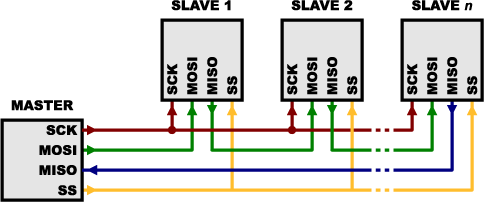
\includegraphics[width=0.75\textwidth]{spi_4_wires.png}
    \caption{An implementation of a 4-wire SPI with $n$ slaves \cite{SparkFunSpi}}
    \label{figure:4}
  \end{figure}
\end{enumerate}

%%%%%%%%%%%%%%%%%%%%%%%%%%%%%%%%%%%%%%%%%%%%%%%%%%%%%%%%%%%%%%%%%%%%%%%%%%%%%%%%
% Appendix
%%%%%%%%%%%%%%%%%%%%%%%%%%%%%%%%%%%%%%%%%%%%%%%%%%%%%%%%%%%%%%%%%%%%%%%%%%%%%%%%
\section*{Appendix} \label{section:Appendix}

\begin{center}
  \textbf{lab5.qsf} (Pin Assignment)
\end{center}

\inputminted[breaklines, firstline=38, fontfamily=tt, fontsize=\small, frame=lines, framesep=1.5em, linenos, numbersep=1.5em, style=vs]{text}{lab5/lab5.qsf}

\begin{center}
  \textbf{SpiTopLevel.sv}
\end{center}

\inputminted[breaklines, fontfamily=tt, fontsize=\small, frame=lines, framesep=1.5em, linenos, numbersep=1.5em, style=vs]{systemverilog}{lab5/SpiTopLevel.sv}

\begin{center}
  \textbf{Spi.sv}
\end{center}

\inputminted[breaklines, fontfamily=tt, fontsize=\small, frame=lines, framesep=1.5em, linenos, numbersep=1.5em, style=vs]{systemverilog}{lab5/Spi.sv}

\begin{center}
  \textbf{Parser.sv}
\end{center}

\inputminted[breaklines, fontfamily=tt, fontsize=\small, frame=lines, framesep=1.5em, linenos, numbersep=1.5em, style=vs]{systemverilog}{lab5/Parser.sv}

\begin{center}
  \textbf{Decoder.sv}
\end{center}

\inputminted[breaklines, fontfamily=tt, fontsize=\small, frame=lines, framesep=1.5em, linenos, numbersep=1.5em, style=vs]{systemverilog}{lab5/Decoder.sv}

%%%%%%%%%%%%%%%%%%%%%%%%%%%%%%%%%%%%%%%%%%%%%%%%%%%%%%%%%%%%%%%%%%%%%%%%%%%%%%%%
%Bibliography
%%%%%%%%%%%%%%%%%%%%%%%%%%%%%%%%%%%%%%%%%%%%%%%%%%%%%%%%%%%%%%%%%%%%%%%%%%%%%%%%
\bibliographystyle{ieeetr}
\bibliography{references}

\end{document}
